% Preamble
% Estructura del documento a editar

\documentclass[]{article} 
% Se recomienda cargar los paquetes que se utilizarán
\usepackage{graphicx} % paquete de gráficas
\usepackage{float} % Paquete de posicionamiento
\usepackage{subfigure}
\usepackage{amsmath}
\usepackage{amssymb}



%opening
\title{ejemplo artículo en latex}
\author{Seminario 2021}

\begin{document}

\maketitle

\begin{abstract}
Abstract 250-300 palabras
\end{abstract}

\section{Introducción}
información sección

Tomado de \cite{Rasmunssen05}

\section{Materiales y Métodos}

\subsection{Base de datos}

\subsubsection{DB1}

\subsubsection{DB2}

Como se muestra en la figura \ref{fig:img1}, las imágenes en JPEG tienen poca resolución debido a la compresión.\\

Esto sería otra frase.

\begin{figure}[H]
	\centering
	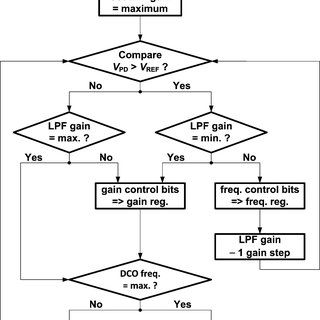
\includegraphics[width=0.2\linewidth]{img/img1}
	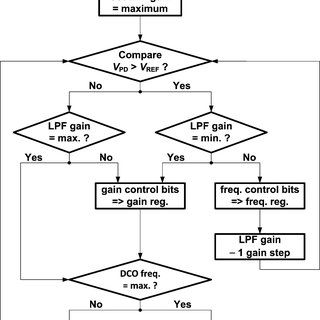
\includegraphics[width=0.2\linewidth]{img/img1}
	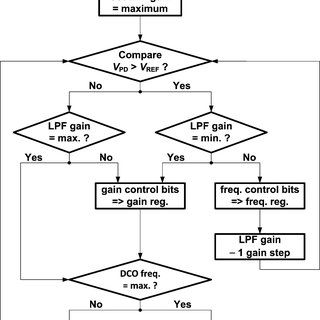
\includegraphics[width=0.2\linewidth]{img/img1}\\
	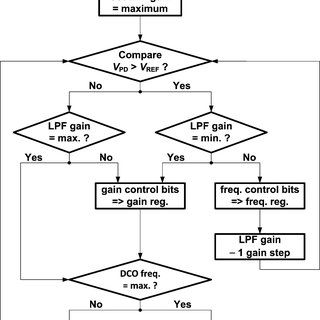
\includegraphics[width=0.2\linewidth]{img/img1}
	\caption{Ejemplo de carga de una imagen JPEG.}
	\label{fig:img1}
\end{figure}


\subsection{Ecuaciones}

Ecuaciones en línea $x = 5 + b^2$

\begin{align}
\hat{\mathbf{x}} = \mathbf{Ax}+\mathbf{Bu}
\label{eq:SS}
\end{align}

La ecuación \eqref{eq:SS} muestra una ec.

\begin{align*}
\hat{\mathbf{x}} = \mathbf{Ax}+\mathbf{Bu}
\label{eq:SS}
\end{align*}


\begin{align}
\nabla \times \mathbf{E}=-\frac{\partial \mathbf{B}}{\partial t}
\end{align}


\begin{align}
\frac{\partial^{2} B}{\partial \lambda^{2}}=\mu_{0} \epsilon_{0} \frac{\partial^{2} B}{\partial t^{2}}
\end{align}

\begin{align}
\log p(\mathbf{f} \mid X) &=-\frac{1}{2} \mathbf{f}^{T} K^{-1} \mathbf{f}  \notag\\
 &-\frac{1}{2} \log |K|-\frac{n}{2} \log 2 \pi
\end{align}

XXXXXXXXXXXXXXx $\log p(\mathbf{f} \mid X)=-\frac{1}{2} \mathbf{f}^{T} K^{-1} \mathbf{f}-\frac{1}{2} \log |K|-\frac{n}{2} \log 2 \pi$ XXXXXXXXXXXXXXx

\section{Resultados y Discusión}

La figura \ref{fig:Comparacion} muestra XXXXXXXXXX.

\begin{figure}
	\centering
	\subfigure[Imagen PNG]{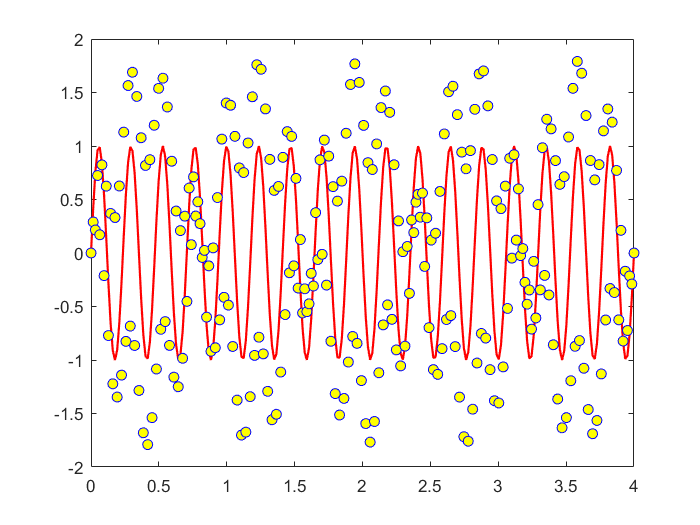
\includegraphics[width=0.45\textwidth]{img/img2}}
	\subfigure[Imagen PDF]{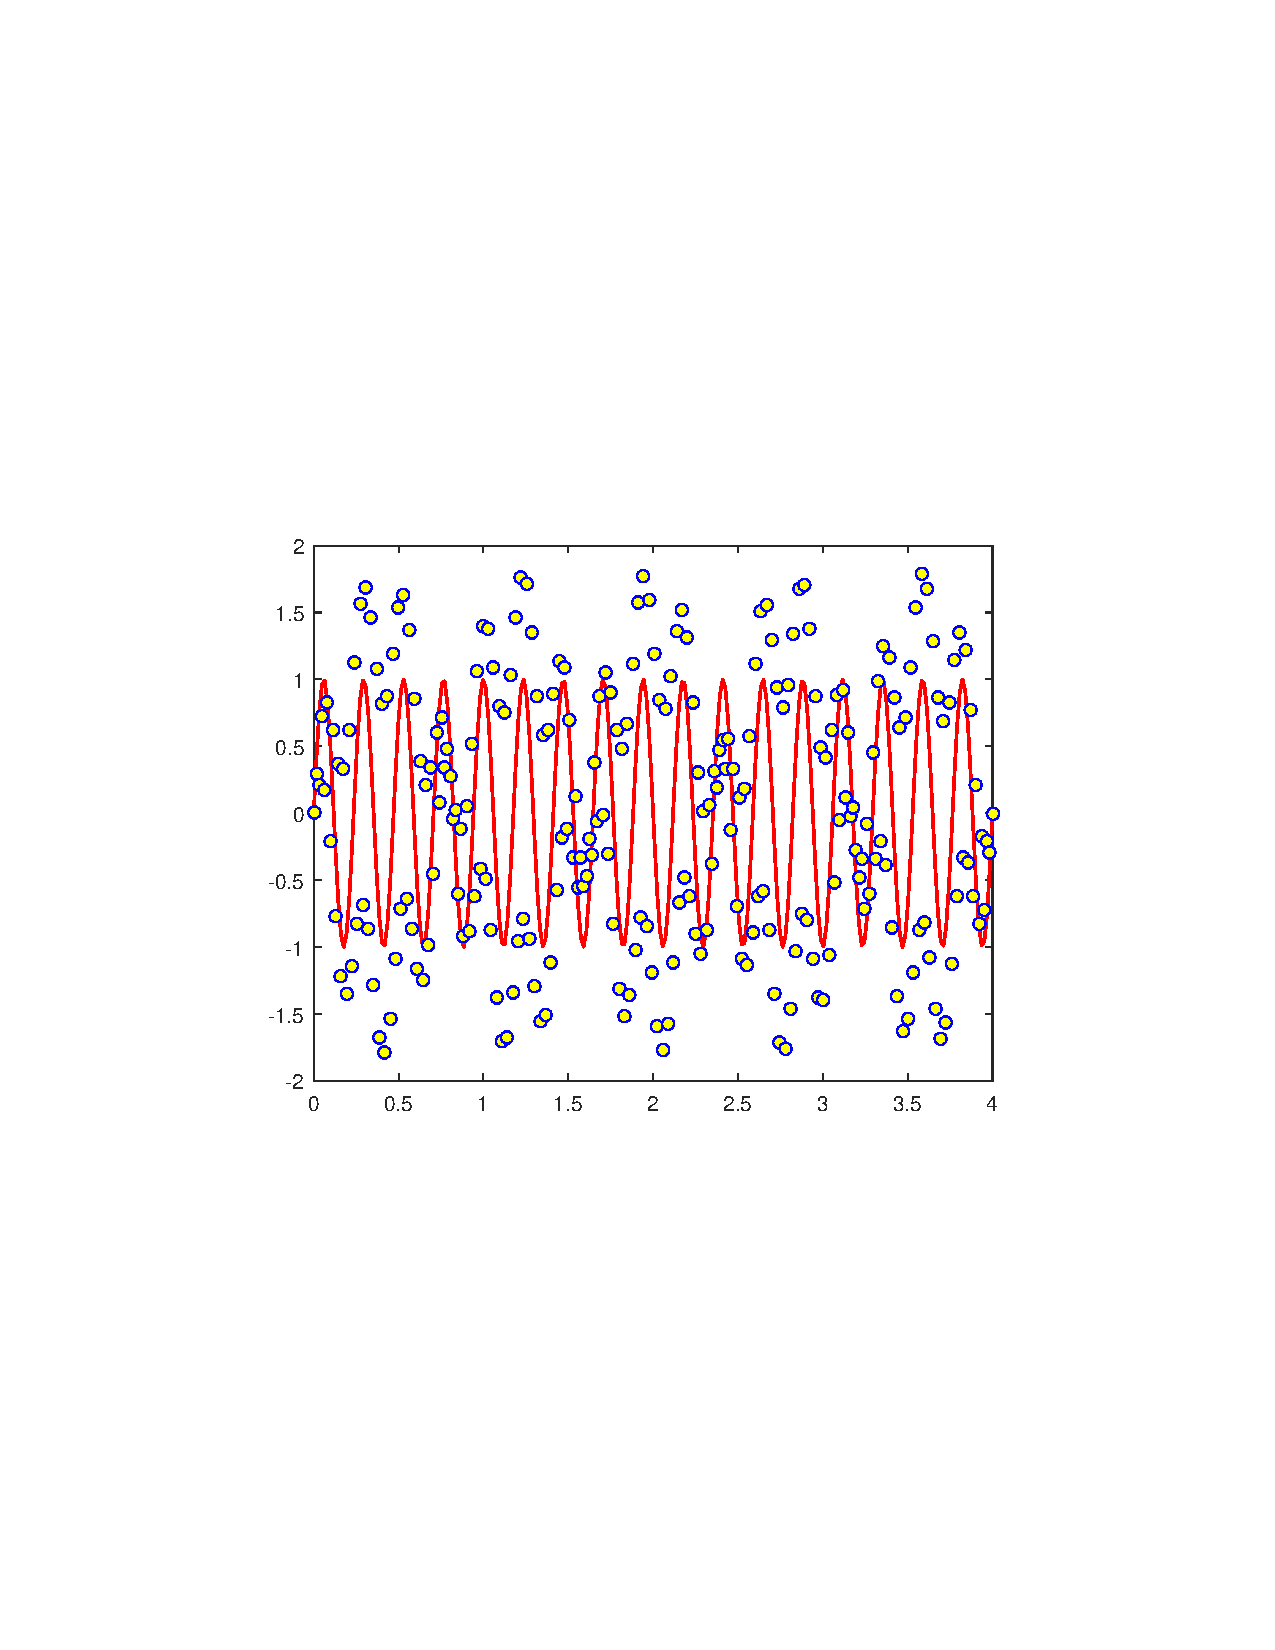
\includegraphics[width=0.41\textwidth]{img/img3}}
	\caption{Comparación de dos figuras en diferentes formatos.}
	\label{fig:Comparacion}
\end{figure}

\section{Conclusiones}


% Para crear la refrencias
% 1. Estilo de la bibliografía
\bibliographystyle{Plain}
\bibliography{biblio}

\end{document}
